\documentclass[a4paper,12pt]{article}
\usepackage{fullpage}
\usepackage[T1]{fontenc}
\usepackage{amsmath}
\usepackage{amssymb}
\usepackage[utf8]{inputenc}
\usepackage{color}
\usepackage{authblk}
\usepackage{todonotes}
\usepackage{caption}
\usepackage{url}
\usepackage{float}
\usepackage{sectsty}
\usepackage{pdfpages}
\usepackage[section]{placeins}
\DeclareCaptionFont{white}{\color{white}}
\DeclareCaptionFormat{listing}{\colorbox{gray}{\parbox{\textwidth}{#1#2#3}}}
\captionsetup[lstlisting]{format=listing,labelfont=white,textfont=white}

\usepackage{setspace}
\usepackage[toc,page]{appendix}
\usepackage{framed}
\usepackage{geometry}

\usepackage{alltt}
\usepackage{subfig}

% Change section fonts
\allsectionsfont{\sffamily}

% For code box
\usepackage{xcolor}
\usepackage{listings}
\usepackage{caption}
\DeclareCaptionFont{white}{\color{white}}
\DeclareCaptionFormat{listing}{%
  \parbox{\textwidth}{\colorbox{gray}{\parbox{\textwidth}{#1#2#3}}\vskip-4pt}}
  \captionsetup[lstlisting]{format=listing,labelfont=white,textfont=white}
  \lstset{frame=lrb,xleftmargin=\fboxsep,xrightmargin=-\fboxsep}
% End code box

\usepackage{cite}

% General parameters, for ALL pages:
\renewcommand{\topfraction}{0.9}	% max fraction of floats at top
\renewcommand{\bottomfraction}{0.8}	% max fraction of floats at bottom
% Parameters for TEXT pages (not float pages):
\setcounter{topnumber}{2}
\setcounter{bottomnumber}{2}
\setcounter{totalnumber}{4} % 2 may work better
\setcounter{dbltopnumber}{2} % for 2-column pages

\addtolength{\topmargin}{0.5in}

\usepackage{fancyvrb}

\usepackage{tikz} \usetikzlibrary{trees}
\usepackage{hyperref} % should always be the last package

% useful colours (use sparingly!):
\newcommand{\blue}[1]{{\color{blue}#1}}
\newcommand{\green}[1]{{\color{green}#1}}
\newcommand{\red}[1]{{\color{red}#1}}

% useful wrappers for algorithmic/Python notation:
\newcommand{\length}[1]{\text{len}(#1)}
\newcommand{\twodots}{\mathinner{\ldotp\ldotp}} % taken from clrscode3e.sty
\newcommand{\Oh}[1]{\mathcal{O}\left(#1\right)}

% useful (wrappers for) math symbols:
\newcommand{\Cardinality}[1]{\left\lvert#1\right\rvert}
\newcommand{\Ceiling}[1]{\left\lceil#1\right\rceil}
\newcommand{\Floor}[1]{\left\lfloor#1\right\rfloor}
\newcommand{\Iff}{\Leftrightarrow}
\newcommand{\Implies}{\Rightarrow}
\newcommand{\Intersect}{\cap}
\newcommand{\Sequence}[1]{\left[#1\right]}
\newcommand{\Set}[1]{\left\{#1\right\}}
\newcommand{\SetComp}[2]{\Set{#1\SuchThat#2}}
\newcommand{\SuchThat}{\mid}
\newcommand{\Tuple}[1]{\langle#1\rangle}
\newcommand{\Union}{\cup}
\usetikzlibrary{positioning,shapes,shadows,arrows}
\providecommand{\keywords}[1]{\textbf{\textit{Keywords: }} #1}

\title{\textbf{Specification: Designing a Virtual Security Layer for Cloud Content}}
\author{Lukas Klingsbo}

\begin{document}

\maketitle

\setcounter{tocdepth}{3}
\tableofcontents

\clearpage
\pagenumbering{arabic}
\setcounter{page}{1}
\section{Background}
This work will be done at the company Uprise (Dragarbrunnsgatan 36C, Uppsala). 
The goal of this project is to design and develop a local access control layer 
for files and views in a content distribution network.
This should make handling of content safer and make it easier to have control 
over the security settings of groups of files and will also make 
it possible to enforce local (as in not on the CDN) auth and audit logging.

\section{Description}
The project should design and possibly develop a system where it is possible 
to set different types of access to different clusters of virtual files. 
For example, the access control could be divided into three groups:
\begin{itemize}
  \item Very secret - Only accessible from white listed IP addresses
  \item Secret - Only accessible from authenticated users with the correct access
  \item Public - Accessible by anybody
\end{itemize}
The security rules put in place should not be hard coded, but possible to update 
and extend. When a file is set to a belong to one of these groups it should not be static, 
it should be possible to, at a later stage, assign it to another group.

A virtual file, as described in the beginning of the description, is a form of pointer 
connected to some meta-data that points at an actual file in the filesystem or remote 
service. One ``physical'' file can be referenced by many virtual files.

It should also be possible to create so called views which a group 
of files are added to, which then have their own security settings.
A view is a subset of files, and a view can be a view of another view and then 
only contain files which is in contained in the parent view. 
A file can be a part of several views that then in their turn have different 
security settings. The system should then be able to determine what the correct 
security setting for the actual file is or if it needs to create several versions 
of the file. 

For example, which security rules should take precedence if a file, lets call it 
``Test.jpg'', is uploaded to a CDN once, but is contained in two views 
with different security settings. If then Test.jpg is changed in one of the views, 
but is not supposed to be changed in the other, how is that handled and how is 
it determined when a change should propagate through the whole system or when it 
should just create a new version of it in the current virtual view.
\vspace{12pt}
\\
More things to examine:
\begin{itemize}
    \item A way to dynamically switch a single or a group of files security settings has 
to be examined as the storage method of the files usually will be distributed.
    \item To make sure you are handling the correct file previews has to be shown in the system.
    \item Access to the system should be configured in a modular sense, one module could be 
LDAP.
\end{itemize}

\begin{figure}[htp] \centering{
    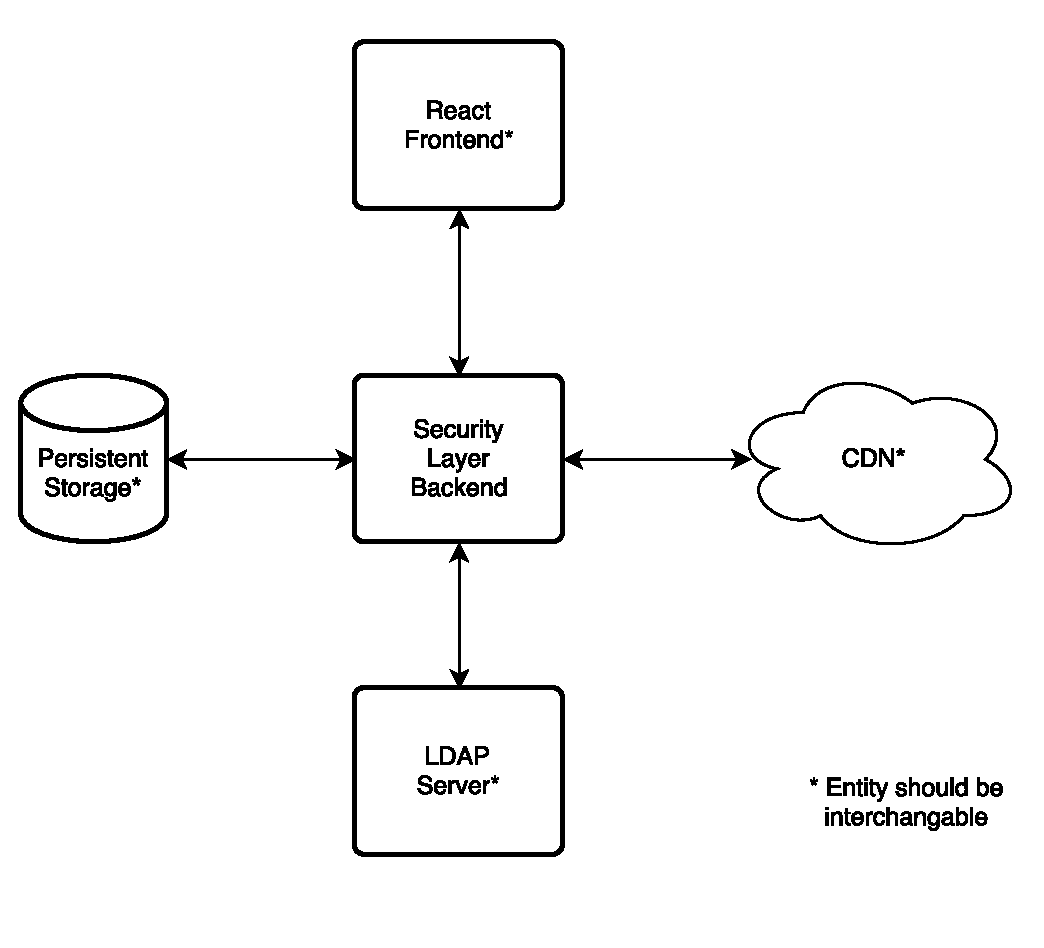
\includegraphics[scale=0.5]{overview.pdf}}
    \caption{System Overview}
    \label{fig:overview}
\end{figure}
If looking at Figure~\ref{fig:overview}, the component that this work is supposed to specifically 
design is the Security Layer in the middle, everything else should be interchangeable. The persistent 
storage will most likely be a database which keeps track of the files and security settings. 
The CDN could be any service with a rougher security system which needs to be more 
fine grained for assets. The LDAP server in the figure can be any form of authentication service so that 
wont need to be handled in the security layer. The React front-end is for handling files and 
security settings in the back-end, it should be possible to write any front-end for it.

\newpage
\section{Methods}
\begin{itemize}
  \item The design will be well evaluated in the sense of security and technical usability
  \item The prototype/system will be developed in Scala and React
  \item A literature study will be done to find more relevant litterature once the specification is accepted 
  \item The proof should be an informal paper proof or if time is sufficient a proper proof should be done in a model checker
  \item Results from the informal proof will be evaluated and documented
  \item The implementation will be evaluated with existing security tools, it needs to be researched which these tools will be
      \item Results from these tools and that are relevant to the report will be added in an appendix
  \item Everything relevant in the work process, from problems that occured to final results, will be documented in the report
  \item The code will have its own documentation separated from the report 
  \item The prototype/system will be released under an open source license
  \item A work station and desk space will be provided by Uprise
\end{itemize}

\section{Relevant Courses}
\begin{itemize}
  \item Computer Networks I (1DT052)
  \item Computer Networks II (1DT074)
  \item Distributed Systems (1DT064)
  \item Secure Computer Systems I (1DT072)
  \item Secure Computer Systems II (1DT073)
  \item Process Oriented Programming (1DT083)
\end{itemize}

\section{Delimitations}
If the project is easier than expected it could be expanded by looking into 
automatically doing simpler image analysis to find images that are about to 
be assigned to the incorrect category, for example a ``Very secret'' image 
that is about to be published as ``Public''.

It is possible to do delimitation of the core research question as the project 
proceeds, but it will most likely not be needed as the research question is 
quite concise.
\newpage
\section{Time Plan}
Note that this is just a rough time plan that will change during the course of 
the project when the circumstances change.
There will rarely be one task at a time, but rather a lot of the tasks will be 
overlapping.
\begin{itemize}
  \item A few days - Properly setting up the work station
  \item 2 weeks - Literature study and obtaining relevant books etc
  \item 20 weeks - Writing the report should be done pretty much 
  throughout the whole project
  \item 1 week - Analyze the current system for managing the CDN assets
  \item 1 week - Analyze what has been done earlier regarding the 
  subject and determine if anything is useful for this project
  \item 3 weeks - Define system mechanism and model
  \item 3 weeks - Analyse system mechanism and model (this item will overlap with the definition)
  \item 3 weeks - Informal proof (or formal if time is sufficient) of the systems mechanism and model
  \item 8 weeks - Implement a prototype/system
      \subitem 1 week - defining and developing backend API
      \subitem 2 weeks - define a basic set of extendable security rules
      \subitem <1 week - investigate and implement "physical" file handler
      \subitem <1 week - implement simple persistant storage for meta data
      \subitem 1-2 weeks - implement authentication interface
      \subitem <1 week - implement CDN interface
      \subitem 2 weeks - implement user interface
  \item 1 weeks - Test security of implementation, if only a prototype is developed the security should only be analysed in theory
\end{itemize}

The interfaces does not have to have anything real connected to them, it just needs 
to be possible to hook up services to them.



\section{References}
    One possibility to connect the security layer to:

\url{http://docs.aws.amazon.com/AmazonCloudFront/latest/DeveloperGuide/private-content-signed-cookies.html}

    \end{document}
